\chapter{Experimental and Results}\label{chap:results}
This chapter reports the results of the experiments designed in Chapter~3 and answers the four research questions of Section~1.3 in order. Every number is computed from the records of the runs and from the test predictions saved by each run. All results use the data of Section~\ref{sec:data_collection}, with the Normal traffic extracted under the export settings of the dataset authors.

\section{Introduction}\label{sec:res_intro}

The run ledger holds 1,237 rows for 431 configurations, most of them run with three seeds. A one-seed trial run re-executed the base matrix from scratch and reproduced 53 of 53 ledger rows exactly; only the byte counts of secure aggregation runs differ, by up to 31 bytes, because they depend on random keys. The macro-F1 recomputed from the saved test predictions equals the ledger value to within $8 \times 10^{-17}$. The $\varepsilon$ of the 42 DP-SGD runs was recomputed with the separate accountant of Section~\ref{subsec:privacy_accounting}; the largest relative difference from the reported value is 1.22\%, below the limit of 10\%.

Four conventions apply to every table and figure below.
\begin{itemize}
    \item \textbf{Scores:} utility is measured on the locked real test split of 30,000 rows (5,000 per class) and is written as mean $\pm$ standard deviation over the seeds $\{0, 1, 2\}$, with $\mathrm{ddof} = 0$.
    \item \textbf{Classifier:} a row labelled with a generator reports the classifier, RF or MLP, that had the higher macro-F1 on the real validation split. Where both are shown, the classifier is named.
    \item \textbf{Privacy budget:} $\varepsilon$ is stated at record level (one packet) with $\delta = 10^{-5}$ unless a unit is named. For distributed noise it is the value when every gateway adds its share; the value for fewer honest gateways is given separately.
    \item \textbf{Verdicts:} ``better'', ``worse'' and ``no effect'' have the meaning of Equation~\eqref{eq:decision_rule}. A dagger ($\dagger$) marks a verdict that changes under the bootstrap over whole TCP streams.
\end{itemize}

\subsubsection*{Names Used in This Chapter}
Three configurations are the main ones of the framework: MG-eps1 is MGs-eps1, MG-eps5 is MGr-eps5, and MG-eps10 is MGs-eps10. MGs, MGr, MGd and MGl are the variants of Table~\ref{tab:mg_variants}. On the CVAE side, B3 has no protection, M2 adds SecAgg$^+$, M1 adds DP-SGD, and M3 combines both. The suffix ``o'' (M1o, M3o) marks the settings searched at full federated scale in round O1. For each $\varepsilon$, the CVAE row used against FedDP-Marginal is the best valid CVAE route on validation: M1-eps1, M3o-eps5 and M1o-eps10.

\subsubsection*{Organisation}
Section~\ref{sec:res_data} presents the data as they were used, the leakage checks, the settings selected on validation, and the consolidated scorecard. Section~\ref{sec:res_analysis} analyses the results per research question. Section~\ref{sec:res_interpretation} explains the patterns, Section~\ref{sec:res_literature} compares them with published work, and Section~\ref{sec:res_implications} draws the practical consequences.

\clearpage
\section{Presentation of Data}\label{sec:res_data}

\subsection{The Data as Used}
The dataset holds 39,000,601 packets (Table~\ref{tab:dataset_composition}), of which 130,500 are sampled into the training, validation and test splits under the quotas of Table~\ref{tab:quota}. The real test split comes from 11 capture groups and 20,485 TCP streams. The training split has 77,106 TCP streams and 147 capture groups, so a stream contributes 1.15 rows on average, while one capture contributes up to 1,277 rows. No TCP stream appears in more than one split.

Figure~\ref{fig:res_partition} shows the non-IID partition of the first seed. With Dirichlet $\alpha = 0.5$, the five gateways hold between 3,666 and 33,618 rows in this seed, and over the three seeds the client sizes range from 2,862 to 69,578 rows. Several gateways hold almost no rows of some rare sub-classes. Client 1, for example, has no SYN\_DoS row. This is the situation the federation is meant to address.

\begin{figure}[htbp]
\centering
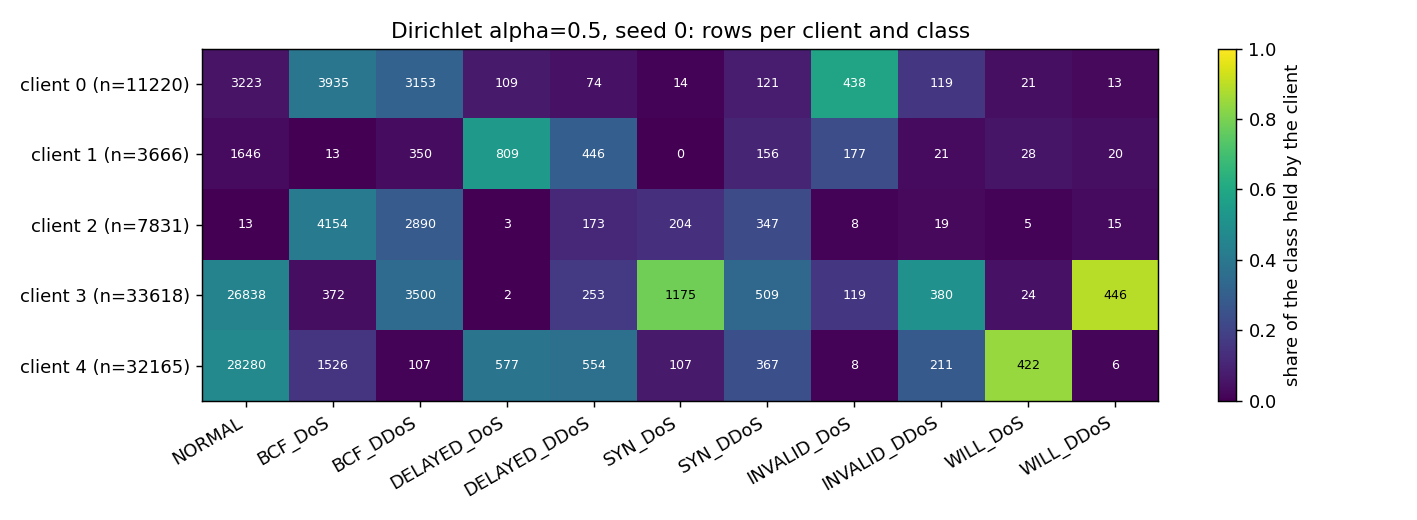
\includegraphics[width=\textwidth]{graphics/chapter4/partition_alpha0.5_seed0.png}
\caption{Non-IID partition of the training rows over the five gateways (Dirichlet $\alpha = 0.5$, seed 0). Each cell gives the number of rows of a sub-class at a gateway; the colour gives the share of that sub-class held by the gateway.}
\label{fig:res_partition}
\end{figure}

\subsection{Leakage and Label-Reliability Checks}
Table~\ref{tab:res_leakage} gives the outcome of the five checks of Table~\ref{tab:leakage_checks}. Only one flag was raised.

\begin{table}[htbp]
\centering
\small
\caption{Results of the leakage and label-reliability checks (Random Forest with 100 trees, validation split, three seeds)}
\label{tab:res_leakage}
\begin{tabularx}{\textwidth}{lXL{3.2cm}}
\toprule
\textbf{Check} & \textbf{Result} & \textbf{Decision} \\
\midrule
C1 & Five columns are empty in some sub-classes and populated in others. Of these, only \texttt{requested\_qos}, \texttt{will\_message\_length} and \texttt{will\_topic\_length} are model features, with a presence of at most 0.166 & Kept: they follow from the protocol \\
\midrule
C2 & Macro-F1 from the 12 \texttt{\_is\_na} flags alone: $0.1775 \pm 0.0000$, against 0.167 for chance & Not flagged (threshold 0.5) \\
\midrule
C3 & Best single column: \texttt{frame\_length\_on\_wire\_2}, macro-F1 0.2972. Best per-class F1 from one column: 0.4134 (\texttt{tcp\_segment\_len}, INVALID) & Not flagged (threshold 0.9) \\
\midrule
C4 & Five-fold macro-F1 by random row 0.5394, by stream 0.5365, by capture group 0.5308. Gaps: random minus group $+0.0086$, random minus stream $+0.0029$ & Not flagged (threshold 0.05) \\
\midrule
C5 & DoS against DDoS, macro-F1: BCF 0.5915, DELAYED 0.6151, WILL 0.6841, INVALID 0.7871, SYN 0.9630 & BCF flagged (threshold 0.6); the others are separable \\
\bottomrule
\end{tabularx}
\end{table}

Three facts from these checks shape the rest of the chapter. First, no column gives the class away, so the task is not artificially easy. Second, the detection task is hard: an RF on real data reaches a validation macro-F1 of $0.4482 \pm 0.0009$, or $0.5002 \pm 0.0002$ with class-balanced weights. Third, the time columns carry much of the signal. Without \texttt{irtt}, \texttt{time\_delta\_from\_previous\_displayed\_frame} and \texttt{time\_since\_first\_frame\_in\_this\_tcp\_stream}, the class-balanced macro-F1 falls to $0.3464$, and the F1 of DELAYED falls from 0.418 to 0.001.

Check C5 also bears on the six-class merge. Only BCF falls below the threshold, so the merge does not rest on the two variants being inseparable. It is a design choice that keeps enough rows per class, and Section~\ref{subsec:res_robustness} reports the eleven-class results for reference.

\subsection{References on Real Data}
Table~\ref{tab:res_references} gives the references. They train on the pooled real split and therefore need what the threat model forbids. They mark how far a detector can go on these features when pooling is allowed.

\begin{table}[htbp]
\centering
\small
\caption{References trained on the pooled real training split (TRTR)}
\label{tab:res_references}
\begin{tabularx}{\textwidth}{Xccc}
\toprule
\textbf{Reference} & \textbf{Macro-F1} & \textbf{Balanced accuracy} & \textbf{Rare-class recall} \\
\midrule
B0, real data only, RF & $0.448 \pm 0.000$ & 0.481 & 0.285 \\
B0, real data only, MLP & $0.343 \pm 0.006$ & 0.418 & 0.190 \\
B1a, class weights, RF & $0.496 \pm 0.000$ & 0.518 & 0.355 \\
B1b, SMOTE, RF & $0.505 \pm 0.002$ & 0.516 & 0.381 \\
B1b, SMOTE, MLP & $0.477 \pm 0.014$ & 0.485 & 0.365 \\
\bottomrule
\end{tabularx}
\end{table}

The B0 RF recalls NORMAL at 0.964 and BCF at 0.780, but only DELAYED at 0.231, SYN at 0.472, INVALID at 0.161 and WILL at 0.276. Each of the rare classes is hard to separate packet by packet, even for a model trained on all the real rows.

\subsection{Settings Selected on Validation}
Table~\ref{tab:res_settings} lists the settings selected for FedDP-Marginal over three seeds on the validation split, together with the CVAE routes tuned in round O1 on one seed. The two generator families were not tuned with the same effort per candidate, an asymmetry stated in Section~\ref{subsec:hpo}.

\begin{table}[htbp]
\centering
\small
\caption{Settings selected on the validation split}
\label{tab:res_settings}
\begin{tabularx}{\textwidth}{cXcc}
\toprule
$\boldsymbol{\varepsilon}$ & \textbf{FedDP-Marginal setting} & \textbf{Coarse bins} & \textbf{Budget split $\boldsymbol{\omega}$} \\
\midrule
1 & MGs & 16 & $(0.3, 0.1, 0.6)$ \\
5 & MGr: inverse-variance fusion, IPF, smoothing $\alpha = 0.1$, root by noisy MI & 16 & $(0.15, 0.05, 0.8)$ \\
10 & MGs & 8 & $(0.5, 0.1, 0.4)$ \\
\bottomrule
\end{tabularx}
\end{table}

At $\varepsilon = 5$ and $\varepsilon = 10$, the two best FedDP-Marginal candidates differ by only 0.000016 and 0.000008 on validation. Both gaps are below the weight of one validation packet in the macro-F1, which is $1/(6 \times 2{,}000) = 0.00008$. The selected settings at these budgets should therefore be read as members of a tied group, not as clear winners.

\subsection{Consolidated Scorecard}
Table~\ref{tab:res_scorecard} gathers the main configurations. Appendix~\ref{app:scorecard} holds all rows of the scorecard. Figure~\ref{fig:res_f1_by_config} shows the matrix of the two classifiers under TAug and TSTR.

\begin{table}[htbp]
\centering
\small
\setlength{\tabcolsep}{4pt}
\caption{Main configurations under TSTR. An asterisk marks byte counts estimated from the number of cells, because MGl runs in process.}
\label{tab:res_scorecard}
\begin{tabularx}{\textwidth}{Xcccccccc}
\toprule
\textbf{Config.} & \textbf{Clf.} & $\boldsymbol{\varepsilon}$ & \textbf{Macro-F1} & \textbf{Binary F1} & \textbf{Rare recall} & \textbf{MB/round} & \textbf{Rounds} & \textbf{MB/run} \\
\midrule
B3 (CVAE, no protection) & MLP & $\infty$ & $0.413 \pm 0.005$ & 0.904 & 0.361 & 4.20 & 30 & 126.1 \\
M2 (CVAE, SecAgg$^+$) & MLP & $\infty$ & $0.419 \pm 0.008$ & 0.896 & 0.361 & 6.37 & 30 & 191.1 \\
M1-eps1 & MLP & 1 & $0.176 \pm 0.008$ & 0.750 & 0.068 & 0.56 & 30 & 16.9 \\
M3o-eps5 & MLP & 5 & $0.254 \pm 0.013$ & 0.814 & 0.132 & 0.91 & 15 & 13.6 \\
M1o-eps10 & MLP & 10 & $0.275 \pm 0.015$ & 0.799 & 0.146 & 1.45 & 50 & 72.4 \\
\midrule
MGl-eps1 (local DP) & RF & 1 & $0.267 \pm 0.021$ & 0.774 & 0.117 & 0.38* & 3 & 1.13* \\
MGl-eps5 (local DP) & RF & 5 & $0.397 \pm 0.006$ & 0.825 & 0.279 & 0.35* & 3 & 1.05* \\
MGl-eps10 (local DP) & MLP & 10 & $0.406 \pm 0.015$ & 0.828 & 0.277 & 0.31* & 3 & 0.94* \\
\midrule
MGs-eps1 (distributed) & RF & 1 & $0.366 \pm 0.018$ & 0.813 & 0.231 & 0.18 & 3 & 0.53 \\
MGr-eps5 (distributed) & MLP & 5 & $0.425 \pm 0.004$ & 0.824 & 0.301 & 0.17 & 3 & 0.51 \\
MGs-eps10 (distributed) & MLP & 10 & $0.433 \pm 0.004$ & 0.843 & 0.301 & 0.16 & 3 & 0.48 \\
\midrule
MGp-nodp (plain Flower) & MLP & $\infty$ & $0.459 \pm 0.007$ & 0.885 & 0.367 & 0.11 & 3 & 0.34 \\
MGs-nodp (SecAgg$^+$) & MLP & $\infty$ & $0.459 \pm 0.007$ & 0.885 & 0.367 & 0.16 & 3 & 0.47 \\
\bottomrule
\end{tabularx}
\end{table}

\begin{figure}[htbp]
\centering
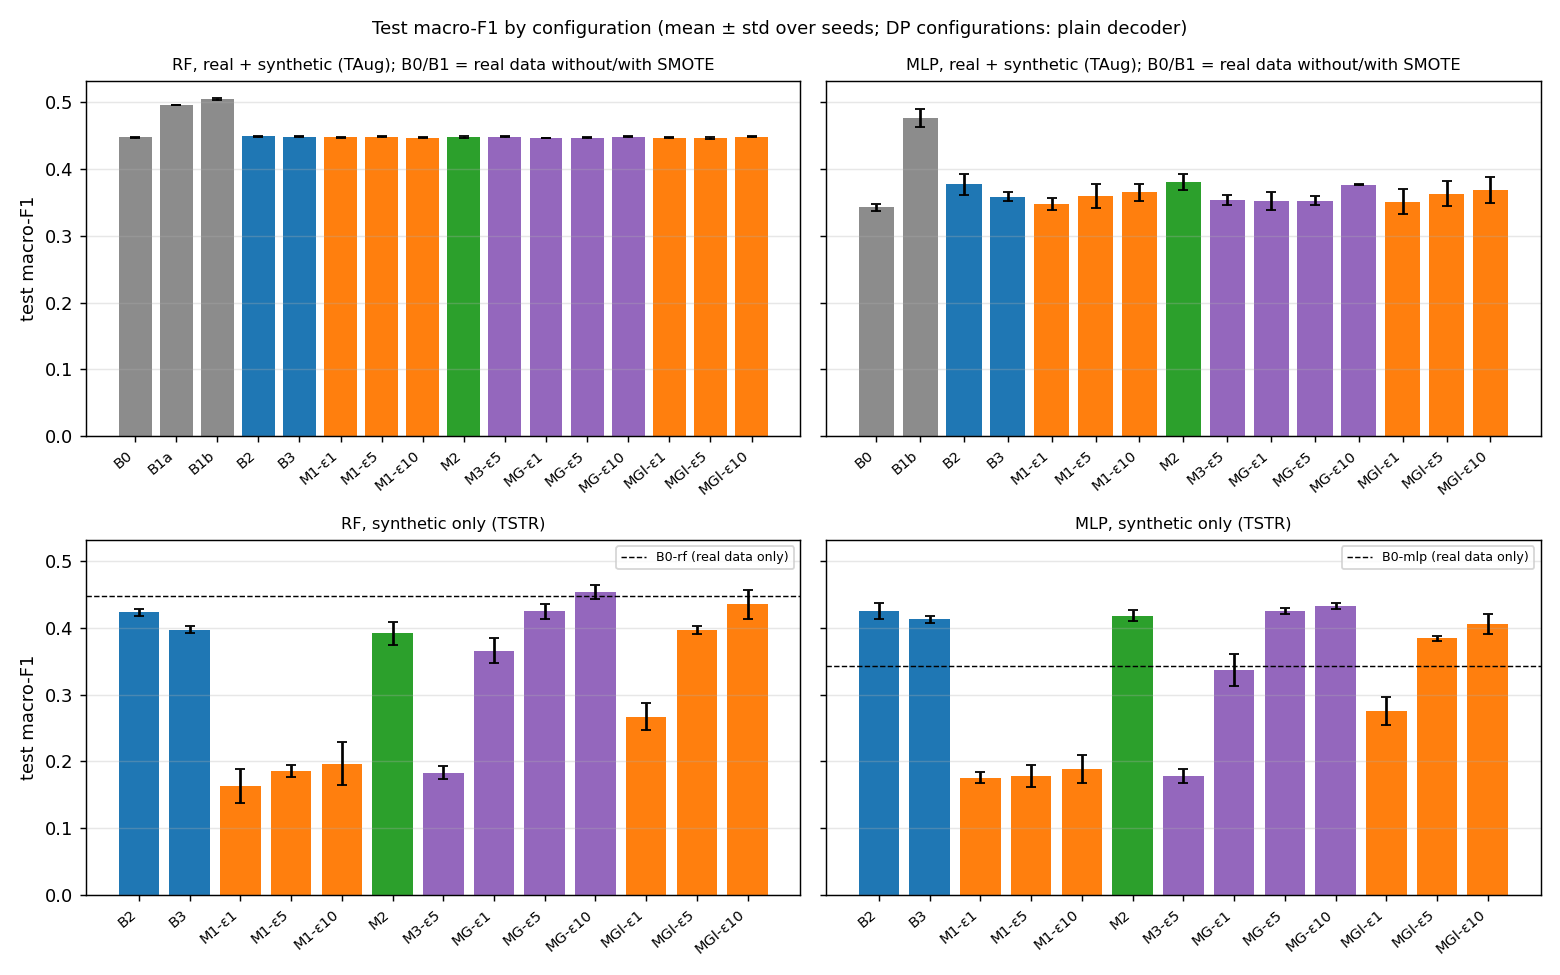
\includegraphics[width=\textwidth]{graphics/chapter4/f1_by_config.png}
\caption{Test macro-F1 by configuration and classifier. Upper row: real plus synthetic data (TAug) and the real-data references. Lower row: synthetic data only (TSTR), with the B0 level as a dashed line. MG-$\varepsilon$ denotes the main FedDP-Marginal configurations.}
\label{fig:res_f1_by_config}
\end{figure}

Figure~\ref{fig:res_tstr_eps} draws the TSTR macro-F1 of the main routes against the privacy budget. The curves of FedDP-Marginal lie above those of the CVAE at every budget.

\begin{figure}[htbp]
\centering
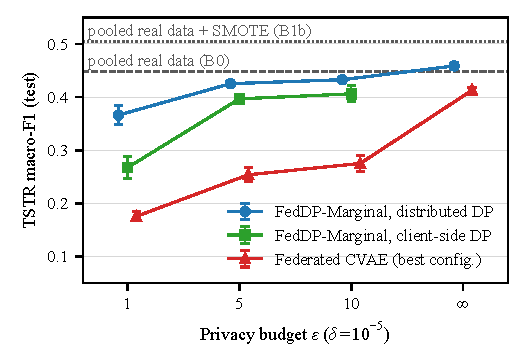
\includegraphics[width=0.8\textwidth]{graphics/chapter4/tstr_vs_eps.pdf}
\caption{TSTR macro-F1 against the privacy budget $\varepsilon$ for the main routes (mean over three seeds, with the seed standard deviation), with the reference levels on pooled real data.}
\label{fig:res_tstr_eps}
\end{figure}

\FloatBarrier
\clearpage
\section{Analysis of Results}\label{sec:res_analysis}

\subsection{RQ1: Utility of the Synthetic Data for the IDS}\label{subsec:res_rq1}

\subsubsection*{Synthetic Data Alone (TSTR)}
Where the raw traffic cannot be pooled, the classifier has only the synthetic data. Table~\ref{tab:res_scorecard} shows what remains. Without DP, FedDP-Marginal reaches 0.459 and the CVAE route reaches 0.413. With DP, FedDP-Marginal keeps 0.366, 0.425 and 0.433 at $\varepsilon = 1, 5, 10$, close to the RF on pooled real data (0.448). The SMOTE and class-weight references on pooled real data stay higher, at 0.505 and 0.496.

A TSTR score at or above the B0 level does not mean that synthetic data are better than real data. Red flag F2 of the protocol (TSTR above TRTR) was triggered for the MLP, whose B0 reference is low because it is trained on the imbalanced split, while the synthetic set holds 5,000 rows of every class. Against a class-balanced real reference, the flag disappears: no TSTR score reaches B1b-RF (0.505) or B1b-MLP (0.477).

\subsubsection*{Adding Synthetic Rows to Pooled Real Data (TAug and TAugR)}
Table~\ref{tab:res_taug} gives the gain from adding synthetic rows to the pooled real data. For the RF, 2 of the 13 generators pass the decision rule and the largest gain is $+0.0012$, while SMOTE gains $+0.0575$ and class weights $+0.0483$. For the MLP, 9 of the 13 generators pass, with a largest gain of $+0.0378$, against $+0.1339$ for SMOTE. The recall of the four rare classes under the RF moves by at most 0.007 for any generator and class, against $+0.070$ and $+0.096$ (mean over the four classes) for class weights and SMOTE.

The targeted variant does no better. In the scorecard, the gain of TAugR over B0 lies between $-0.001$ and $+0.001$ for every generator, with the ratio chosen on validation.

\begin{table}[htbp]
\centering
\small
\setlength{\tabcolsep}{4pt}
\caption{TAug: difference of test macro-F1 against real data only (B0), with the 95\% paired bootstrap interval}
\label{tab:res_taug}
\begin{tabularx}{\textwidth}{Xllll}
\toprule
\textbf{Configuration} & \textbf{RF: $\Delta$ [95\% CI]} & \textbf{Verdict} & \textbf{MLP: $\Delta$ [95\% CI]} & \textbf{Verdict} \\
\midrule
B1a (reference) & $+0.0483$ $[+0.0449, +0.0514]$ & better & not applicable & \\
B1b (reference) & $+0.0575$ $[+0.0538, +0.0613]$ & better & $+0.1339$ $[+0.1289, +0.1384]$ & better \\
\midrule
B2 & $+0.0012$ $[+0.0001, +0.0024]$ & better & $+0.0343$ $[+0.0319, +0.0365]$ & better \\
B3 & $+0.0011$ $[+0.0000, +0.0023]$ & better $\dagger$ & $+0.0162$ $[+0.0140, +0.0184]$ & better \\
M1-eps1 & $-0.0000$ $[-0.0010, +0.0008]$ & no effect & $+0.0049$ $[+0.0030, +0.0069]$ & no effect \\
M1-eps5 & $+0.0011$ $[+0.0002, +0.0020]$ & no effect & $+0.0170$ $[+0.0153, +0.0186]$ & no effect \\
M1-eps10 & $-0.0006$ $[-0.0015, +0.0004]$ & no effect & $+0.0223$ $[+0.0201, +0.0243]$ & better \\
M2 & $+0.0005$ $[-0.0005, +0.0016]$ & no effect & $+0.0378$ $[+0.0353, +0.0406]$ & better \\
M3-eps5 & $+0.0005$ $[-0.0004, +0.0014]$ & no effect & $+0.0114$ $[+0.0097, +0.0129]$ & better \\
MG-eps1 & $-0.0010$ $[-0.0020, +0.0001]$ & no effect & $+0.0096$ $[+0.0079, +0.0112]$ & no effect \\
MG-eps5 & $-0.0008$ $[-0.0020, +0.0002]$ & no effect & $+0.0101$ $[+0.0082, +0.0120]$ & better \\
MG-eps10 & $+0.0009$ $[-0.0002, +0.0021]$ & no effect & $+0.0341$ $[+0.0313, +0.0368]$ & better \\
MGl-eps1 & $-0.0004$ $[-0.0014, +0.0006]$ & no effect & $+0.0085$ $[+0.0064, +0.0107]$ & no effect \\
MGl-eps5 & $-0.0012$ $[-0.0022, -0.0001]$ & worse & $+0.0205$ $[+0.0182, +0.0227]$ & better \\
MGl-eps10 & $+0.0011$ $[-0.0000, +0.0022]$ & no effect & $+0.0256$ $[+0.0232, +0.0281]$ & better \\
\bottomrule
\end{tabularx}
\end{table}

\subsubsection*{The CVAE Against the Simple Methods}
TAug with the CVAE (B2 centralised, B3 federated) against class weights and SMOTE gives six comparisons, and all six are worse, with a macro-F1 difference between $-0.1177$ and $-0.0471$ and a rare-class recall difference between $-0.167$ and $-0.068$. When real data can be pooled, the two simple methods are the better choice in this study.

\subsubsection*{What Federation Costs a Non-Private CVAE}
Moving from the centralised CVAE (B2) to five non-IID clients (B3) costs $+0.0257$ $[+0.0225, +0.0291]$ of macro-F1 under TSTR with the RF, which is a relative loss of 6.1\%. Under TSTR with the MLP the cost is $+0.0129$ (3.0\%), and under TAug with the MLP it is $+0.0181$ (4.8\%). TAug with the RF shows no effect ($+0.0001$).

\subsubsection*{Local Augmentation at Each Gateway}
Table~\ref{tab:res_local_aug} shows the setting where synthetic rows give the most. A gateway that has seen little of some classes trains its own RF and receives synthetic rows of the classes it holds fewer than 5,000 rows of. The mean macro-F1 of the 15 client models rises from $0.384 \pm 0.055$ to $0.423$, $0.426$ and $0.427$ with the main FedDP-Marginal configurations. Those are gains of $+0.039$, $+0.042$ and $+0.043$, with 11, 13 and 13 of the 15 client models gaining. Losses are at most 0.005 and gains reach 0.139.

\begin{table}[htbp]
\centering
\small
\caption{Local augmentation at each gateway (RF, 15 client models over 5 clients and 3 seeds, mean $\pm$ standard deviation)}
\label{tab:res_local_aug}
\begin{tabularx}{\textwidth}{Xcccc}
\toprule
\textbf{Training data of a client} & \textbf{Macro-F1} & \textbf{Rare recall} & \textbf{Gain over local} & \textbf{Clients better} \\
\midrule
Local real rows only & $0.384 \pm 0.055$ & 0.297 & n/a & n/a \\
Local + B3 (CVAE, no protection) & $0.425 \pm 0.044$ & 0.311 & $+0.041$ & 15 / 15 \\
Local + M2 (CVAE, SecAgg$^+$) & $0.423 \pm 0.046$ & 0.310 & $+0.039$ & 15 / 15 \\
Local + M1o-eps5 (CVAE, DP) & $0.398 \pm 0.053$ & 0.295 & $+0.014$ & 10 / 15 \\
Local + MG-eps1 & $0.423 \pm 0.045$ & 0.308 & $+0.039$ & 11 / 15 \\
Local + MG-eps5 & $0.426 \pm 0.044$ & 0.311 & $+0.042$ & 13 / 15 \\
Local + MG-eps10 & $0.427 \pm 0.043$ & 0.313 & $+0.043$ & 13 / 15 \\
Local + MGl-eps5 & $0.422 \pm 0.044$ & 0.307 & $+0.038$ & 12 / 15 \\
\bottomrule
\end{tabularx}
\end{table}

\subsubsection*{IDS-Side Options}
Class-probability weights chosen on validation, and the use of all 20,000 synthetic rows per class, act on the classifier and leave the generator unchanged. Their effect depends on the generator. For MG-eps1, the RF rises from 0.365 to 0.406 and the rare-class recall from 0.235 to 0.311; the MLP rises from 0.344 to 0.414 with both options. For MG-eps5 and MG-eps10, the changes are small and mixed in sign. The weights correct the tendency of an IDS trained on synthetic rows to predict NORMAL too often. They need labelled real validation data, and they must be chosen again for another class mix, so they are reported as an option only.

\subsubsection*{The Alternative of Training the Detector Directly}
A federation that needs only a detector can train the classifier itself by FedAvg, with no generator. Table~\ref{tab:res_direct} compares this route with the generators at the same protection. With the first group of settings (DP at each client), the direct MLP is above the CVAE route under DP. With distributed DP, where the noise is split over the gateways as in FedDP-Marginal, the direct MLP (DP-FedSGD) is not different from the framework at $\varepsilon = 1$ and below it at $\varepsilon = 5$ and $\varepsilon = 10$.

\begin{table}[htbp]
\centering
\small
\setlength{\tabcolsep}{4pt}
\caption{The classifier trained directly by federated learning, compared with the generator routes at the same protection (TSTR with the MLP on the generator side)}
\label{tab:res_direct}
\begin{tabularx}{\textwidth}{Xcccl}
\toprule
\textbf{Direct route and protection} & \textbf{Direct MLP} & \textbf{Generator route} & \textbf{$\Delta$ [95\% CI]} & \textbf{Verdict} \\
\midrule
\multicolumn{5}{l}{\emph{Against the CVAE route}} \\
No protection & $0.425 \pm 0.026$ & 0.413 & $+0.012$ $[+0.008, +0.015]$ & no effect \\
SecAgg$^+$ (numerical emulation) & $0.416 \pm 0.021$ & 0.419 & $-0.003$ $[-0.006, +0.000]$ & no effect \\
DP at each client, $\varepsilon = 1$ & $0.245 \pm 0.008$ & 0.176 & $+0.069$ $[+0.066, +0.073]$ & better \\
DP at each client, $\varepsilon = 5$ & $0.276 \pm 0.022$ & 0.178 & $+0.098$ $[+0.093, +0.102]$ & better \\
DP at each client, $\varepsilon = 10$ & $0.290 \pm 0.024$ & 0.189 & $+0.101$ $[+0.097, +0.106]$ & better \\
\midrule
\multicolumn{5}{l}{\emph{Against FedDP-Marginal, noise split over the gateways in both routes}} \\
DP-FedSGD, $\varepsilon = 1$ & $0.350 \pm 0.010$ & 0.337 & $+0.013$ $[+0.010, +0.016]$ & no effect \\
DP-FedSGD, $\varepsilon = 5$ & $0.369 \pm 0.001$ & 0.425 & $-0.057$ $[-0.060, -0.053]$ & worse \\
DP-FedSGD, $\varepsilon = 10$ & $0.389 \pm 0.011$ & 0.433 & $-0.043$ $[-0.047, -0.040]$ & worse \\
\bottomrule
\end{tabularx}
\end{table}

The two routes cost very different amounts of communication. DP-FedSGD needs 2,593 model rounds and about 7.7\,GB in total over the clients (an estimate from the bytes per parameter measured for M2), against three rounds and 0.48 to 0.53\,MB for FedDP-Marginal. Its epsilon with a single honest gateway grows to 3.1, 58.6 and 142.0, against 2.4, 14.2 and 33.1 for FedDP-Marginal. Without noise, the same recipe reaches $0.467 \pm 0.008$, against $0.459$ for FedDP-Marginal without DP. That difference of $+0.008$ $[+0.004, +0.012]$ passes the rule. Federated SMOTE, with no generator and no protection, reaches $0.445 \pm 0.016$.

\subsubsection*{Answer to RQ1}
When real data can be pooled, synthetic data do not improve the IDS in any way that matters in this study, and class weights or SMOTE do better. When raw traffic cannot be pooled, the data from FedDP-Marginal keep a TSTR macro-F1 between 0.366 and 0.433 at $\varepsilon$ from 1 to 10, which is 82\% to 97\% of the RF on pooled real data. The most useful role is local augmentation, where a gateway with few rows of some classes gains about 0.04 of macro-F1.

\subsection{RQ2: FedDP-Marginal Against the Federated CVAE}\label{subsec:res_rq2}

\subsubsection*{Utility at the Same Budget}
Table~\ref{tab:res_rq2} applies the decision rule to the difference between FedDP-Marginal and the best CVAE route at each budget. All 12 comparisons are ``better'' under both the record and the stream bootstrap.

\begin{table}[htbp]
\centering
\small
\setlength{\tabcolsep}{4pt}
\caption{FedDP-Marginal minus the best CVAE route with DP (TSTR on the real test split). All verdicts are ``better'' under both bootstraps.}
\label{tab:res_rq2}
\begin{tabularx}{\textwidth}{cXccc}
\toprule
$\boldsymbol{\varepsilon}$ & \textbf{Comparison} & \textbf{$\Delta$ macro-F1 [95\% CI]} & \textbf{Largest seed sd} & \textbf{$\Delta$ rare recall [95\% CI]} \\
\midrule
1 & MGl-eps1 $-$ M1-eps1 & $+0.092$ $[+0.088, +0.095]$ & 0.021 & $+0.049$ $[+0.046, +0.053]$ \\
1 & MGs-eps1 $-$ M1-eps1 & $+0.191$ $[+0.187, +0.195]$ & 0.018 & $+0.163$ $[+0.160, +0.168]$ \\
5 & MGl-eps5 $-$ M3o-eps5 & $+0.143$ $[+0.139, +0.147]$ & 0.013 & $+0.147$ $[+0.143, +0.152]$ \\
5 & MGr-eps5 $-$ M3o-eps5 & $+0.171$ $[+0.167, +0.176]$ & 0.013 & $+0.169$ $[+0.163, +0.174]$ \\
10 & MGl-eps10 $-$ M1o-eps10 & $+0.131$ $[+0.127, +0.135]$ & 0.015 & $+0.131$ $[+0.126, +0.136]$ \\
10 & MGs-eps10 $-$ M1o-eps10 & $+0.158$ $[+0.154, +0.162]$ & 0.015 & $+0.155$ $[+0.150, +0.160]$ \\
\bottomrule
\end{tabularx}
\end{table}

The local variant (MGl) gives the cleanest comparison, because it adds noise at each gateway exactly as the CVAE does, so the difference comes from the generator and not from the noise split. Moving to distributed noise then adds about 0.03 to 0.10 of macro-F1 at the same $\varepsilon$.

\subsubsection*{What DP Costs Each Generator}
DP costs the CVAE far more than it costs FedDP-Marginal. Against the CVAE without DP with the same plain decoder, M1 at $\varepsilon = 1, 5, 10$ is worse in 11 of 12 comparisons, and the loss in TSTR macro-F1 runs up to 58\%. Against its own $\varepsilon = \infty$, FedDP-Marginal loses $-0.076$ (RF) and $-0.122$ (MLP) at $\varepsilon = 1$, $-0.017$ and $-0.033$ at $\varepsilon = 5$, and changes by $+0.012$ (RF) and $-0.026$ (MLP) at $\varepsilon = 10$.

Re-tuning the CVAE per budget at full federated scale (round O1) did not close this gap. It lifts the best valid CVAE route to 0.254 at $\varepsilon = 5$ and 0.275 at $\varepsilon = 10$, against 0.178 and 0.189 for the first search. At $\varepsilon = 1$, the setting chosen on validation does worse on the test split (0.167 for M1o-eps1 with the RF), so the baseline M1-eps1 remains the best CVAE route there.

\subsubsection*{Per-Class Behaviour and the Working Hypotheses}
Table~\ref{tab:res_per_class} and Figure~\ref{fig:res_per_class} break the scores down by class.

\begin{table}[htbp]
\centering
\small
\setlength{\tabcolsep}{4pt}
\caption{Test F1 per class (mean over three seeds; classifier chosen on validation)}
\label{tab:res_per_class}
\begin{tabularx}{\textwidth}{Xcccccc}
\toprule
\textbf{Configuration} & \textbf{NORMAL} & \textbf{BCF} & \textbf{DELAYED} & \textbf{SYN} & \textbf{INVALID} & \textbf{WILL} \\
\midrule
B0, RF (real data only) & 0.521 & 0.559 & 0.362 & 0.560 & 0.256 & 0.428 \\
B1b, RF (SMOTE) & 0.548 & 0.585 & 0.450 & 0.556 & 0.381 & 0.511 \\
\midrule
B3 (CVAE, no protection) & 0.623 & 0.318 & 0.418 & 0.426 & 0.336 & 0.356 \\
M1-eps1 & 0.339 & 0.319 & 0.102 & 0.095 & 0.042 & 0.156 \\
M3o-eps5 & 0.510 & 0.391 & 0.125 & 0.115 & 0.096 & 0.287 \\
M1o-eps10 & 0.499 & 0.408 & 0.119 & 0.238 & 0.199 & 0.188 \\
\midrule
MGs-eps1 & 0.523 & 0.457 & 0.250 & 0.407 & 0.181 & 0.378 \\
MGr-eps5 & 0.530 & 0.459 & 0.311 & 0.445 & 0.377 & 0.429 \\
MGs-eps10 & 0.539 & 0.482 & 0.321 & 0.444 & 0.419 & 0.391 \\
MGs-nodp & 0.585 & 0.485 & 0.379 & 0.429 & 0.432 & 0.440 \\
\bottomrule
\end{tabularx}
\end{table}

\begin{figure}[htbp]
\centering
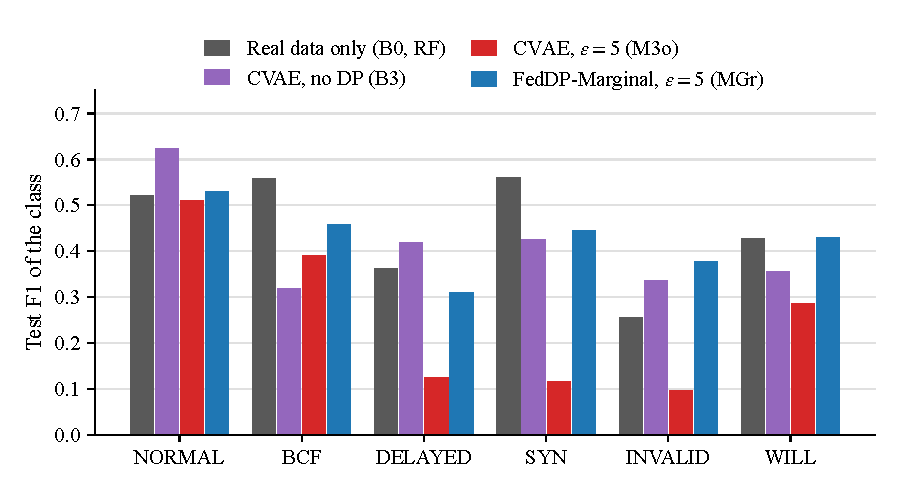
\includegraphics[width=0.85\textwidth]{graphics/chapter4/per_class_f1.pdf}
\caption{Test F1 per class for the real-data reference, the CVAE without DP, and the two generator routes at $\varepsilon = 5$.}
\label{fig:res_per_class}
\end{figure}

\textbf{H1} predicted that at $\varepsilon = 1$ the marginal generator would reach a higher class-level F1 on the classes defined by discrete header fields (INVALID, WILL). The point estimates support it: MGs-eps1 minus M1-eps1 is $+0.139$ for INVALID and $+0.222$ for WILL, and both exceed the largest seed standard deviation of the two configurations (0.086 and 0.073). \textbf{H2} predicted the reverse for the volumetric classes (BCF, SYN). The results do not support it: the difference is $+0.138$ for BCF and $+0.312$ for SYN, again in favour of FedDP-Marginal and above the largest seed standard deviation (0.047 for both). Per-class differences were compared with the seed spread only; the paired bootstrap of Section~\ref{subsec:decision_rule} was applied to the macro-F1 and to the mean rare-class recall.

\subsubsection*{Fidelity}
Table~\ref{tab:res_fidelity} gives the fidelity measures. FedDP-Marginal is closer to the real numeric marginals than the CVAE with DP at the same budget: the Wasserstein distance at $\varepsilon = 5$ is 0.037 against 0.194, and at $\varepsilon = 10$ it is 0.049 against 0.176. The distance at $\varepsilon = 5$ is below the one at $\varepsilon = 10$; the two main configurations are not the same variant (MGr with fusion and 16 bins at $\varepsilon = 5$, MGs with 8 bins at $\varepsilon = 10$), so the two values are not points on one curve.

No generator produces rows that a classifier cannot tell from real ones. The C2ST AUC is between 0.9995 and 1.0000 in every row, DP or not, deep or marginal. Utility for a detector therefore does not imply that the rows look real.

\begin{table}[htbp]
\centering
\small
\caption{Fidelity of the synthetic sets (mean over classes and seeds)}
\label{tab:res_fidelity}
\begin{tabularx}{\textwidth}{Xcccc}
\toprule
\textbf{Configuration} & \textbf{Wasserstein} & \textbf{Jensen--Shannon} & \textbf{Correlation distance} & \textbf{C2ST AUC} \\
\midrule
B3 (CVAE, no protection) & 0.1029 & 0.0024 & 0.0633 & 0.9997 \\
M1-eps1 & 0.2352 & 0.0159 & 0.1649 & 1.0000 \\
M1-eps5 & 0.1944 & 0.0128 & 0.1390 & 1.0000 \\
M1-eps10 & 0.1755 & 0.0103 & 0.1244 & 0.9999 \\
\midrule
MG-eps1 & 0.1941 & 0.0232 & 0.1691 & 0.9998 \\
MG-eps5 & 0.0374 & 0.0003 & 0.0581 & 0.9997 \\
MG-eps10 & 0.0489 & 0.0025 & 0.0740 & 0.9995 \\
\midrule
MGl-eps1 & 0.2691 & 0.0376 & 0.2191 & 0.9999 \\
MGl-eps5 & 0.1132 & 0.0094 & 0.1244 & 0.9998 \\
MGl-eps10 & 0.0722 & 0.0059 & 0.0995 & 0.9997 \\
\bottomrule
\end{tabularx}
\end{table}

\subsubsection*{Answer to RQ2}
At the same $(\varepsilon, \delta)$, FedDP-Marginal achieves a higher TSTR macro-F1 and a higher rare-class recall than the federated CVAE with DP at every tested budget, by $+0.092$ to $+0.191$ of macro-F1. It also has a higher score without DP ($+0.044$ RF, $+0.046$ MLP against B3). The remaining advantage of the non-private CVAE is the binary F1, 0.904 against 0.885 for FedDP-Marginal without DP.

\subsection{RQ3: Overhead, Granularity and Honest Gateways}\label{subsec:res_rq3}

\subsubsection*{Cost of Secure Aggregation}
Table~\ref{tab:res_secagg} gives the overhead. Time is compute time on one machine and network latency is not measured. SecAgg$^+$ adds little to either route. Its effect on utility is negligible: for the CVAE route, 7 of 8 comparisons with the unprotected route show no effect and one is better ($+0.0216$, TAug with the MLP). For FedDP-Marginal the secure sum equals the exact sum, so the runs with and without SecAgg$^+$ release the same tables and the same synthetic data at every seed, and the TSTR difference is 0.000.

\begin{table}[htbp]
\centering
\small
\caption{Measured overhead of secure aggregation}
\label{tab:res_secagg}
\begin{tabularx}{\textwidth}{Xccc}
\toprule
\textbf{Pair} & \textbf{Time} & \textbf{Volume per round} & \textbf{Ratios (time, bytes)} \\
\midrule
M2 / B3 (CVAE, no DP) & 2.18 s vs 1.95 s & 60.6 vs 40.0 bytes per parameter & 1.12, 1.52 \\
M3-eps5 / M1-eps5 (CVAE, DP) & 3.83 s vs 3.76 s & 64.7 vs 40.0 bytes per parameter & 1.02, 1.62 \\
MGs-nodp / MGp-nodp & 21.6 s vs 20.4 s (run) & 0.158 vs 0.114 MB & 1.06, 1.39 \\
\bottomrule
\end{tabularx}
\end{table}

DP-SGD itself is the expensive part of the CVAE route: its median time per round is 3.76\,s, against 1.95\,s for B3, a ratio of 1.93. Over a whole run with $K = 5$, FedDP-Marginal stays at or below 1.33\,MB across all its configurations, while the CVAE routes take from 8.4 to 191\,MB. Figure~\ref{fig:res_traffic} shows the trade-off between total traffic and detection.

\begin{figure}[htbp]
\centering
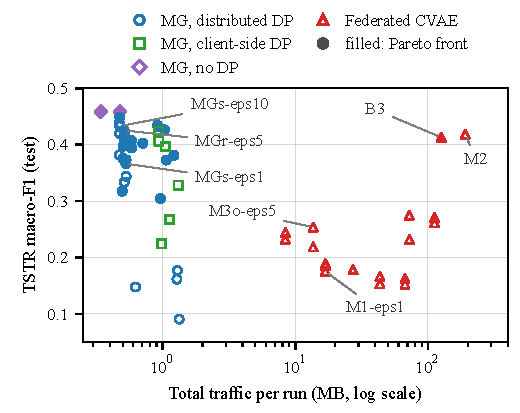
\includegraphics[width=0.8\textwidth]{graphics/chapter4/f1_vs_traffic.pdf}
\caption{TSTR macro-F1 against the total traffic of a run. Filled markers belong to the Pareto front.}
\label{fig:res_traffic}
\end{figure}

\subsubsection*{Protected Unit}
Table~\ref{tab:res_units} shows the cost of moving the guarantee from one packet to a larger unit. Protecting a TCP stream costs 0.03 to 0.05 of macro-F1, since 90\% of the streams hold a single row. Protecting a whole capture is not usable on this data. The macro-F1 falls to 0.09 to 0.18, because only a few thousand rows can be kept (3,675 at $m = 25$).

\begin{table}[htbp]
\centering
\small
\caption{TSTR macro-F1 by protected unit (rows kept in brackets when capped)}
\label{tab:res_units}
\begin{tabularx}{\textwidth}{cXXX}
\toprule
$\boldsymbol{\varepsilon}$ & \textbf{Packet} & \textbf{TCP stream} & \textbf{Capture} \\
\midrule
1 & $0.366 \pm 0.018$ & $0.334 \pm 0.025$ ($m = 1$; 77,106) & $0.091 \pm 0.037$ ($m = 25$; 3,675) \\
5 & $0.425 \pm 0.004$ & $0.376 \pm 0.007$ ($m = 1$; 77,106) & $0.177 \pm 0.020$ ($m = 50$; 7,350) \\
10 & $0.433 \pm 0.004$ & $0.382 \pm 0.004$ ($m = 2$; 80,244) & $0.148 \pm 0.021$ ($m = 100$; 14,000) \\
\bottomrule
\end{tabularx}
\end{table}

\subsubsection*{Honest Gateways}
With distributed noise, the guarantee holds only if enough gateways add their share. Figure~\ref{fig:res_honest} draws the effective $\varepsilon$ as a function of the number of honest gateways. It grows from 5 to 14.2 at the MGr-eps5 setting when one gateway alone remains honest. The trend worsens with more clients: at $\varepsilon = 5$ with one honest gateway, the value is 25.4 for $K = 10$ and 49.9 for $K = 20$.

\begin{figure}[htbp]
\centering
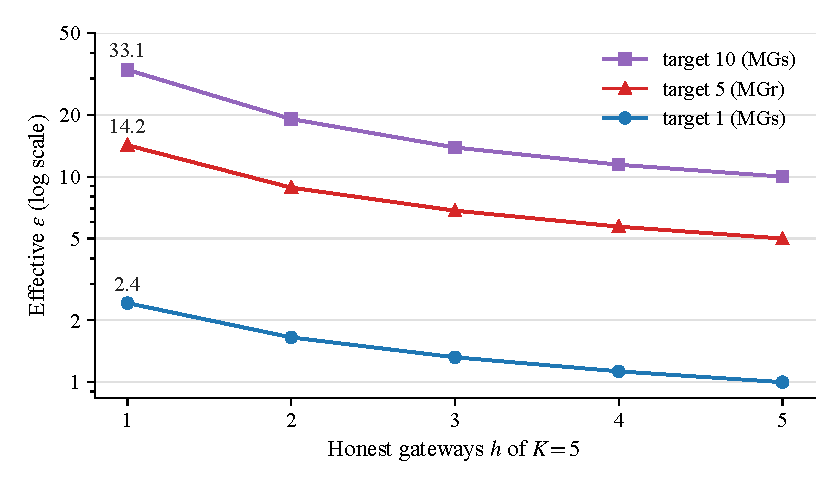
\includegraphics[width=0.75\textwidth]{graphics/chapter4/eps_by_honest.pdf}
\caption{Effective $\varepsilon$ as a function of the number of honest gateways $h$, for $K = 5$ and calibration at $t = K$.}
\label{fig:res_honest}
\end{figure}

Table~\ref{tab:res_threshold} gives the effect of calibrating the noise for $t$ honest gateways instead of $K$. Each gateway then adds $1/t$ of the noise. Changing $t$ from 5 to 3 moves the macro-F1 by $-0.005$ to $+0.016$, and changing it to 2 moves it by $-0.022$ to $+0.000$, while the $\varepsilon$ with every gateway honest falls by 24\% to 44\%. On this data, the extra noise of a smaller $t$ is nearly free in utility. This holds for $K = 5$ only.

\begin{table}[htbp]
\centering
\small
\caption{Effect of the honest-gateway threshold $t$ ($K = 5$)}
\label{tab:res_threshold}
\begin{tabularx}{\textwidth}{cc Xccc}
\toprule
\textbf{Target $\varepsilon$} & $\boldsymbol{t}$ & \textbf{TSTR macro-F1} & \textbf{$\varepsilon$ ($t$ honest)} & \textbf{$\varepsilon$ (all honest)} & \textbf{$\varepsilon$ (one honest)} \\
\midrule
1 & 5 & $0.366 \pm 0.018$ & 1.00 & 1.00 & 2.4 \\
1 & 3 & $0.373 \pm 0.029$ & 1.00 & 0.76 & 1.8 \\
1 & 2 & $0.344 \pm 0.013$ & 1.00 & 0.61 & 1.5 \\
\midrule
5 & 5 & $0.425 \pm 0.004$ & 5.00 & 5.00 & 14.2 \\
5 & 3 & $0.420 \pm 0.009$ & 5.00 & 3.72 & 10.1 \\
5 & 2 & $0.425 \pm 0.011$ & 5.00 & 2.94 & 7.6 \\
\midrule
10 & 5 & $0.433 \pm 0.004$ & 10.00 & 10.00 & 33.1 \\
10 & 3 & $0.449 \pm 0.005$ & 10.00 & 7.14 & 22.3 \\
10 & 2 & $0.420 \pm 0.004$ & 10.00 & 5.59 & 15.9 \\
\bottomrule
\end{tabularx}
\end{table}

\subsubsection*{Empirical Privacy Checks}
All duplicate rates are at most 0.0007, and all distance ratios lie between 0.85 and 0.93, inside the heuristic thresholds (at most 0.01 and at least 0.5). These two checks detect only near-copies.

Membership inference on the synthetic set stays between 0.488 and 0.494 for every generator, including B3 without DP. The attack did not pass its positive control on an over-fitted CVAE (AUC 0.510), so an AUC close to 0.5 here only says that no synthetic row is a near-copy of a training row. On a generator that copies its members, the same attack reaches 0.981 without noise and 0.526 with noise of 0.2.

A second attack with access to the released CVAE weights passes its positive control, with a calibrated AUC of $0.647 \pm 0.011$ on the CVAE over-fitted on 500 rows. Against the released federated models it gives $0.506 \pm 0.003$ for B3, $0.497 \pm 0.002$ for M1-eps10, $0.499 \pm 0.002$ for M1-eps5, and $0.502 \pm 0.002$ for M1-eps1. It detects nothing in any of them, including the unprotected B3.

The third attack, on the released tables of FedDP-Marginal, is the only one that separates the release without DP from the releases with DP. Table~\ref{tab:res_mia} and Figure~\ref{fig:res_mia} show the result. The positive control, on tables built from 500 records without noise, reaches 0.835. All three drops in AUC against the release without DP pass the bootstrap, and the absolute leakage remains small: 1.91\% true positives at 1\% false positives without DP.

\begin{table}[htbp]
\centering
\small
\caption{Membership inference on the released tables of FedDP-Marginal (calibrated attack, 1,000 bootstrap resamples)}
\label{tab:res_mia}
\begin{tabularx}{\textwidth}{Xccc}
\toprule
\textbf{Release} & \textbf{AUC [95\% CI]} & \textbf{TPR at 1\% FPR} & \textbf{Drop against no DP [95\% CI]} \\
\midrule
No DP (MGs-nodp) & $0.573$ $[0.568, 0.578]$ & 1.91\% & n/a \\
$\varepsilon = 10$ (MGs-eps10) & $0.539$ $[0.534, 0.544]$ & 1.39\% & $0.034$ $[0.029, 0.040]$ \\
$\varepsilon = 5$ (MGr-eps5) & $0.525$ $[0.519, 0.530]$ & 1.14\% & $0.048$ $[0.042, 0.055]$ \\
$\varepsilon = 1$ (MGs-eps1) & $0.515$ $[0.510, 0.520]$ & 1.14\% & $0.059$ $[0.052, 0.065]$ \\
\bottomrule
\end{tabularx}
\end{table}

\begin{figure}[htbp]
\centering
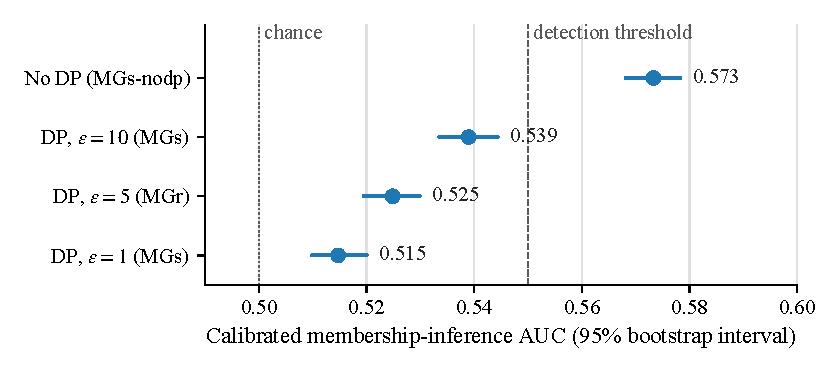
\includegraphics[width=0.75\textwidth]{graphics/chapter4/mia_tables.pdf}
\caption{Calibrated membership-inference AUC on the released tables, with the 95\% bootstrap interval, against the chance level and the heuristic detection threshold.}
\label{fig:res_mia}
\end{figure}

\subsubsection*{Robustness and Sensitivity}\label{subsec:res_robustness}
Table~\ref{tab:res_robustness} reports the branches of Table~\ref{tab:robustness_branches}. Because the distributed variant releases only sums over the clients, its tables do not depend on how the rows are spread: at $\alpha = 0.1$ and $\alpha = 10$, the macro-F1 is the same, 0.398. Its $\varepsilon$ with one honest gateway grows with $K$, while its macro-F1 stays between 0.400 and 0.415. The local variant, which pays the sum of $K$ noises, loses utility as $K$ grows.

\begin{table}[htbp]
\centering
\small
\caption{Robustness of FedDP-Marginal at $\varepsilon = 5$, and the eleven-class mode}
\label{tab:res_robustness}
\begin{tabularx}{\textwidth}{Xccc}
\toprule
\textbf{Setting} & \textbf{TSTR macro-F1} & \textbf{$\varepsilon$ (one honest)} & \textbf{Seeds} \\
\midrule
MGs, main setting ($K = 5$, $\alpha = 0.5$) & $0.408 \pm 0.009$ & 14.2 & 3 \\
MGs, $\alpha = 0.1$ & 0.398 & 14.2 & 1 \\
MGs, $\alpha = 10$ & 0.398 & 14.2 & 1 \\
MGs, $K = 10$ & 0.400 & 25.4 & 1 \\
MGs, $K = 20$ & 0.415 & 49.9 & 1 \\
\midrule
MGl, $K = 5$ & $0.397 \pm 0.006$ & 5.0 & 3 \\
MGl, $K = 10$ & $0.362 \pm 0.017$ & 5.0 & 3 \\
MGl, $K = 20$ & $0.364 \pm 0.021$ & 5.0 & 3 \\
\midrule
Eleven classes, B0, RF (real data only) & $0.336 \pm 0.000$ & n/a & 3 \\
Eleven classes, MGs-eps1 & $0.238 \pm 0.015$ & 2.4 & 3 \\
Eleven classes, MGs-eps5 & $0.284 \pm 0.003$ & 14.2 & 3 \\
Eleven classes, MGs-eps10 & $0.308 \pm 0.004$ & 33.1 & 3 \\
Eleven classes, B3 (CVAE, no protection) & $0.249 \pm 0.018$ & n/a & 3 \\
\bottomrule
\end{tabularx}
\end{table}

Table~\ref{tab:res_sensitivity} repeats the study in five other worlds. Of the ten verdicts compared, six keep the same verdict in every world, and eight keep it across the two alternative choices of test groups (A4). The verdicts that change are mostly small differences close to the seed noise. The comparison between MG-eps5 and the CVAE without DP (B3) under the RF, for example, is ``better'' in the main study and in both A4 worlds, but ``no effect'' under the stream cap A5 and in both quota worlds.

\begin{table}[htbp]
\centering
\small
\caption{Sensitivity worlds: test macro-F1 (mean $\pm$ standard deviation over three seeds)}
\label{tab:res_sensitivity}
\begin{tabularx}{\textwidth}{Xcccc}
\toprule
\textbf{World} & \textbf{B0, RF} & \textbf{B3, TSTR, MLP} & \textbf{MG-eps5, TSTR, RF} & \textbf{MG-eps5, TSTR, MLP} \\
\midrule
Main study & $0.448 \pm 0.000$ & $0.413 \pm 0.005$ & $0.425 \pm 0.012$ & $0.425 \pm 0.004$ \\
A4: other test groups (seed 1) & $0.457 \pm 0.001$ & $0.388 \pm 0.021$ & $0.419 \pm 0.015$ & $0.427 \pm 0.009$ \\
A4: other test groups (seed 2) & $0.462 \pm 0.000$ & $0.371 \pm 0.028$ & $0.416 \pm 0.012$ & $0.429 \pm 0.010$ \\
A5: at most 20 packets per stream & $0.442 \pm 0.001$ & $0.387 \pm 0.019$ & $0.394 \pm 0.006$ & $0.376 \pm 0.006$ \\
A2: rare quotas $\times 6$ & $0.511 \pm 0.000$ & $0.428 \pm 0.015$ & $0.432 \pm 0.007$ & $0.446 \pm 0.013$ \\
A2: rare quotas $\times 0.3$ & $0.405 \pm 0.001$ & $0.386 \pm 0.038$ & $0.388 \pm 0.013$ & $0.372 \pm 0.004$ \\
\bottomrule
\end{tabularx}
\end{table}

\subsubsection*{Answer to RQ3}
SecAgg$^+$ is cheap, at 1.02 to 1.12 times the time and 1.39 to 1.62 times the bytes, and it leaves utility intact. Distributed noise is the main source of the difference between MGs and MGl, but its guarantee depends on how many gateways stay honest. A smaller $t$ gives protection against collusion at almost no cost in utility for $K = 5$. A TCP stream is an affordable unit of protection, whereas a whole capture is not usable on this data.

\subsection{RQ4: Configuration per Deployment Requirement}\label{subsec:res_rq4}

The rule of Section~\ref{subsec:req_rule} takes each requirement of Table~\ref{tab:scenarios} and returns the configuration on its Pareto front with the best value on the requested priority. Table~\ref{tab:res_recommend} gives the outcome. The front of the scorecard holds 18 configurations, 17 of which are FedDP-Marginal variants. The remaining one is B3, retained for its binary F1 and rare-class recall.

\begin{table}[htbp]
\centering
\small
\setlength{\tabcolsep}{4pt}
\caption{Recommended configuration per deployment requirement. The value of $\varepsilon$ is the one that holds under the trust assumed by the requirement.}
\label{tab:res_recommend}
\begin{tabularx}{\textwidth}{lXcccc}
\toprule
\textbf{Scenario} & \textbf{Recommended} & \textbf{Macro-F1} & \textbf{Rare recall} & $\boldsymbol{\varepsilon}$ & \textbf{MB/run} \\
\midrule
\texttt{lab} & MGp-nodp & 0.459 & 0.367 & $\infty$ & 0.3 \\
\texttt{hidden-tables} & MGs-nodp & 0.459 & 0.367 & $\infty$ & 0.5 \\
\texttt{cloud-aggregator} & MGd-eps5 & 0.426 & 0.325 & 5.00 & 1.0 \\
\texttt{consortium} & MGr-t2-eps5 & 0.425 & 0.310 & 7.63 & 0.5 \\
\texttt{strict-privacy} & MGs-t3-eps1 & 0.373 & 0.233 & 1.00 & 0.5 \\
\texttt{low-bandwidth} & MGs-t3-eps10 & 0.449 & 0.346 & 10.00 & 0.5 \\
\texttt{rare-attacks} & MGd-eps5 & 0.426 & 0.325 & 5.00 & 1.0 \\
\texttt{honest-majority} & MGs-t3-eps10 & 0.449 & 0.346 & 10.00 & 0.5 \\
\texttt{gateway-dropout} & MGr-t2-eps5 & 0.425 & 0.310 & 3.94 & 0.5 \\
\texttt{session-privacy} & MGs-strm1-eps5 & 0.397 & 0.310 & 5.00 (stream) & 0.5 \\
\texttt{capture-privacy} & MGr-cap50-eps5 & 0.177 & 0.105 & 5.00 (capture) & 1.3 \\
\bottomrule
\end{tabularx}
\end{table}

Three remarks qualify the table. MGd is a comparator whose Gaussian noise and secure sum are simulated in one process, so a deployment that selects it needs a real implementation of the mechanism. The difference between MGd-eps5 and MGs-t3-eps5 (0.420) lies within the seed noise. The \texttt{capture-privacy} row is the best the data permit, and its macro-F1 of 0.177 does not make it a usable detector.

\subsubsection*{Answer to RQ4}
The choice depends more on trust than on utility. No configuration is best everywhere. Where the operator trusts every party, the versions without DP suffice and give the best detection. Where the aggregator must not see any gateway's tables but the released data stay inside the company, secure aggregation alone meets the requirement. Where a formal guarantee is required, the distributed variants at $\varepsilon = 5$ to 10 give macro-F1 values of 0.408 to 0.449. A demand for $\varepsilon \le 1$ costs about 0.05 to 0.08 in macro-F1 at the same protection level.

\FloatBarrier
\clearpage
\section{Interpretation of Results}\label{sec:res_interpretation}

\subsubsection*{Why FedDP-Marginal Withstands DP Better Than the CVAE}
The privacy budget of the CVAE is consumed through many noisy optimisation steps: each client runs local epochs in each round, and every step composes. FedDP-Marginal spends the budget on three count releases, which are sums with bounded sensitivity. Noise therefore lands directly on what the generator needs. In addition, the CVAE has to learn a joint distribution over 59 columns from noisy gradients, whereas the tree needs only low-order tables. These differences are consistent with the results and with the literature on marginal synthesis, but the study did not isolate them experimentally.

The second structural factor is the noise split. Under secure addition, each gateway can add only $1/K$ of the noise, and the sum still carries the calibrated total. That is valid because each release is a single additive sum. It is not valid for multi-epoch DP-SGD, so SecAgg$^+$ hides the updates of M3 in transit but does not change the noise it needs. This explains why distributed noise raises FedDP-Marginal by up to 0.10 of macro-F1 at the same $\varepsilon$, while M3 and M1 are the same within the noise.

\subsubsection*{Why the Curve Flattens Between $\varepsilon = 5$ and $\varepsilon = 10$}
FedDP-Marginal without DP reaches 0.459, only 0.026 above MG-eps10. Beyond a moderate budget, the limiting factor is what a Chow--Liu tree over 37 attributes, sampled one packet at a time, can represent. The classifier is limited too: the real-data references show that per-packet separation of the rare classes is hard.

\subsubsection*{Why Binary F1 and Macro-F1 Tell Different Stories}
Across the main configurations of Table~\ref{tab:res_scorecard}, the binary F1 ranges from 0.75 to 0.90, and macro-F1 ranges from 0.18 to 0.46. Saying that a packet belongs to an attack is much easier than saying which attack. Most of the difficulty lies in separating the attack families, and part of the literature's high scores comes from reporting only the binary task (Section~\ref{sec:res_literature}).

\subsubsection*{Why Synthetic Rows Add Nothing to Pooled Real Data}
TAug adds synthetic rows to a classifier that already sees all the real rows of every class. A generator trained on those rows, and in particular one that models each packet independently, gives no new information about the boundary between classes. Local augmentation differs, since the client there receives classes it has rarely seen, and this accounts for its gain of about 0.04.

\subsubsection*{Why the Attacks Behave Differently}
The attack on the synthetic set measures near-copies and sees none. The attack on the released CVAE sees nothing either, including in the unprotected B3, which suggests that the training regime of the federated CVAE leaves little membership signal for this attack family. The attack on the tables does see the release without DP, because a count table responds directly to the presence of a record, especially in the sparse cells of rare classes. DP then reduces the signal in a measurable way, and the ordering of the AUC follows $\varepsilon$. Secure aggregation alone does not affect this, since it hides each gateway's tables from the server but not what the released sum reveals.

\subsubsection*{What the Honest-Gateway Results Mean}
With one honest gateway and calibration at $t = K$, the effective $\varepsilon$ is 2.4 to 3.3 times the value claimed for full honesty. The guarantee at $\varepsilon = 10$ becomes 33.1, a value too large to mean much. The threshold $t$ exposes this trade-off and makes it a design decision. It does not remove it.

\subsubsection*{Limits of These Interpretations}
These explanations are consistent with the measured results, but only the comparisons in Section~\ref{sec:res_analysis} were tested. The causal statements in this section were not tested separately, and they apply to one dataset, packet-level features and three seeds.

\clearpage
\section{Comparison with Literature}\label{sec:res_literature}

\subsection{Published Results on the Same Dataset}
Published scores on this dataset are far above the macro-F1 of this study, but they answer other questions, so a score can be read only together with its task, input and split. A study therefore enters Table~\ref{tab:res_lit} only if it trains or tests on this dataset and its full text could be read at the source. Three studies meet both conditions. The search is not systematic: 103 works cite the dataset paper (OpenAlex, snapshot of 2026-11-09), 36 of them mention MQTT and detection, and only the most likely ones were opened.

\begin{table}[htbp]
\centering
\small
\setlength{\tabcolsep}{4pt}
\caption{Published results on the DoS/DDoS-MQTT-IoT dataset, with the task, input and split of each study}
\label{tab:res_lit}
\begin{tabularx}{\textwidth}{L{2.2cm}L{2.6cm}XXL{2.4cm}}
\toprule
\textbf{Study} & \textbf{Task} & \textbf{Input} & \textbf{Split} & \textbf{Reported result} \\
\midrule
Alatram et al.~\cite{alatram2023} & Attack against normal & Packets; the 30-feature list contains source IP, stream index and time columns, and the paper does not say which columns the classifiers received & Not described; 3,654,560 records used & Accuracy of RF 92.69\% to 100\%; no F1 \\
\midrule
Zhang et al.~\cite{zhang2026} & Binary, each attack against benign (DDoS variants of BF, Delay, Sub, WILL) & Packet payload: keywords from 30-packet windows, hashed to 8 integers & Contiguous part of the captures, balanced by selection & F1 (RF) 0.993 to 1.000 \\
\midrule
Parra and Bayas~\cite{parra2026} & Binary, normal against two flooding attacks & TCP flows in 1\,s windows; 4 statistics; no payload & Stratified 70/30 and 5-fold; no separation by capture stated & F1 0.846, AUC 0.876 (hold-out) \\
\midrule
This study & 6 classes, per packet (and the binary tasks below) & Packets; 59 encoded features without source IP, absolute time or stream index & By capture or by block of a capture; 30,000 balanced test packets & Macro-F1: real 0.448, SMOTE 0.505, MG-eps10 0.433; binary F1: 0.786, 0.821, 0.843 \\
\bottomrule
\end{tabularx}
\end{table}

On the closest binary tasks, the saved predictions are re-scored with every attack class counted as ``attack'', with no retraining (Table~\ref{tab:res_lit_binary}). The tasks are close but not identical: the papers train a binary model, while this study reuses its six-class models.

\begin{table}[htbp]
\centering
\small
\caption{Binary F1 on the closest tasks (mean of three seeds)}
\label{tab:res_lit_binary}
\begin{tabularx}{\textwidth}{Xlccc}
\toprule
\textbf{Task} & \textbf{Published (study)} & \textbf{F1} & \textbf{Real data (B1a, RF)} & \textbf{Synthetic, $\varepsilon = 10$} \\
\midrule
Normal / BCF + DELAYED & Parra and Bayas~\cite{parra2026} & 0.846 & 0.837 & 0.832 \\
Normal / BCF & Zhang et al.~\cite{zhang2026} & 1.000 & 0.888 & 0.857 \\
Normal / DELAYED & Zhang et al.~\cite{zhang2026} & 1.000 & 0.738 & 0.723 \\
Normal / INVALID & Zhang et al.~\cite{zhang2026} & 0.993 & 0.786 & 0.728 \\
Normal / WILL & Zhang et al.~\cite{zhang2026} & 0.999 & 0.853 & 0.836 \\
\bottomrule
\end{tabularx}
\end{table}

\subsection{How Much the Protocol Alone Moves a Score}
Table~\ref{tab:res_protocol} measures this directly. The same RF is trained on the same 130,500 sampled packets, and only the split and the identifier columns change.

\begin{table}[htbp]
\centering
\small
\caption{Effect of the split and the identifier columns on the real-data RF (three seeds)}
\label{tab:res_protocol}
\begin{tabularx}{\textwidth}{XXcc}
\toprule
\textbf{Split} & \textbf{Identifier columns added} & \textbf{Macro-F1} & \textbf{Binary F1} \\
\midrule
By capture or block (this study) & None (this study) & $0.448 \pm 0.000$ & $0.786 \pm 0.000$ \\
By capture or block & All of them & $0.842 \pm 0.003$ & $0.974 \pm 0.001$ \\
Random, row by row & None & $0.464 \pm 0.001$ & $0.799 \pm 0.001$ \\
Random, row by row & Source IP & $0.496 \pm 0.001$ & $0.848 \pm 0.001$ \\
Random, row by row & Absolute time, stream index, time since capture start & $0.941 \pm 0.003$ & $0.989 \pm 0.001$ \\
Random, row by row & All of them & $0.939 \pm 0.002$ & $0.987 \pm 0.001$ \\
\bottomrule
\end{tabularx}
\end{table}

The split alone explains little: going from capture to row by row moves the macro-F1 by $+0.017$. Source IP alone adds $+0.032$. The time and stream columns explain the bulk of the gap, adding $+0.476$, because each capture was recorded at its own time and absolute time can identify the capture, and hence the class. A deployed detector cannot rely on such a column, which is why the study removes them. A split by capture does not stop this leak (0.842 with all identifiers), likely because the test rows of 8 of the 11 sub-classes are a block of the same capture as their training rows. These measurements describe this classifier on this data. They do not establish how the classifiers in the cited studies were trained, because those papers do not say, and the study does not claim that their scores are inflated. Differences in task (binary against six classes), input (payload against header features) and identifier columns are enough to make the scores incomparable.

\subsection{Against Federated and Private Data Generation}
None of the studies read combines federated learning, differential privacy and synthetic data on this dataset, so the protected results have no direct published reference. Marginal-based DP synthesis in federated settings already exists. FLAIM~\cite{maddock2024} adapts AIM~\cite{mckenna2024aim} to the federated setting, and CaPS~\cite{pentyala2024} relies on secure multi-party computation. As Chapter~2 notes, these studies evaluate workload error, negative log-likelihood, runtime and communication, on tabular benchmarks that are not intrusion-detection traffic. FLAIM and AIM themselves were not run here, since Private-PGM was not installed, so the study cannot rank FedDP-Marginal against them. To the best of our knowledge, based on a non-systematic search, the contribution here is an evaluation that puts these pieces together: exact distributed DP with Skellam noise~\cite{agarwal2021} through a real SecAgg$^+$ implementation, measured byte counts, the $\varepsilon$ per number of honest gateways, a comparison with a CVAE under the same federation, and a configuration guide per requirement. The study claims no algorithmic novelty.

\clearpage
\section{Implications of the Results}\label{sec:res_implications}

\subsubsection*{For Operators of MQTT Deployments}
A federation of gateways can train a detector without pooling raw traffic. On this data, three short releases of less than 1\,MB in total give a TSTR macro-F1 between 0.366 and 0.433, with a formal guarantee at record level. The cost in bandwidth is low enough for constrained backhaul such as NB-IoT or metered 4G, although the times here are compute times and network behaviour was not measured.

\subsubsection*{For the Design of Privacy-Preserving IDS}
\begin{itemize}
    \item A marginal generator is the better default than a deep generator when a formal guarantee is required at small or moderate $\varepsilon$ on tabular traffic data, in the setting tested.
    \item The $\varepsilon$ must be reported with its unit and its trust assumption. A value of 5 per packet with all gateways honest is not the same guarantee as 14.2 with one honest gateway, or as 5 per TCP stream.
    \item A protected detector can be obtained by another route. If only the detector matters and traffic is not a constraint, the direct federated classifier is a competitor. Where a shareable dataset is needed, or where communication is scarce, the generator route is preferable.
    \item Secure aggregation hides individual gateways from the aggregator at modest cost and does not protect what the final tables reveal. Both mechanisms are needed for different reasons.
\end{itemize}

\subsubsection*{For Evaluation Practice}
The score of an IDS on this dataset moves from 0.448 to 0.941 when only the protocol changes. Reports on this dataset should therefore state the task, the input columns, and the split. Generators should be judged with a positive control for every privacy attack, since an attack at chance says nothing when it cannot detect a deliberately exposed target.

\subsubsection*{What the Results Do Not Allow Us to Claim}
The results do not show that synthetic data improve an IDS when real data can be pooled. They do not show that synthetic rows look real, nor that the framework would behave the same on other traffic. The empirical attacks measure one family of attacks at record level and do not replace the formal guarantee.
